\documentclass[ucs]{beamer}
\usetheme{Frankfurt}
\usepackage[utf8x]{inputenc}
\usepackage[T2A]{fontenc}
\usepackage[english,russian]{babel}

\usepackage{amssymb, amsmath, amsfonts}

% \usepackage{pgfmath}
\usepackage{tikz}
\usetikzlibrary{arrows,fit,positioning,shapes.multipart,shapes.geometric,shapes.symbols,mindmap}

\title{Течения Пуазёйля и Куэтта для разреженного~газа \newline\newline Верификация проекционного метода решения уравнения Больцмана}
\author{Рогозин Олег Анатольевич}
\institute{
	Московский физико-технический институт (государственный университет)
}
\date{}

\newcommand{\dd}{\:\mathrm{d}}
\newcommand{\Kn}{\mathrm{Kn}}
\newcommand{\TV}{\mathrm{TV}}

\begin{document}

\frame{\titlepage}
\begin{frame}
	\frametitle{Содержание}
	\tableofcontents
\end{frame}

\section{Актуальность задачи}

\begin{frame}
	\frametitle{Почему кинетическая теория?}
	\begin{center}
		\vspace{-20pt}
		\begin{tikzpicture}[node distance=4cm,every path/.style={draw,>=latex',very thick},thick,
							block/.style={rectangle,text width=2.6cm,text=white,text badly centered,rounded corners,minimum height=4em}]
			\node[block,fill=blue] (Liu) {Лиувилль\\\(6N\)};
			\node[block,fill=blue,right of=Liu] (Boltz) {Больцман\\6};
			\node[block,fill=blue,right of=Boltz] (NS) {Навье"--~Стокс\\3};
			\draw[->] (Liu.north) to [bend left=60] node[above,text width=4cm,text centered] {молекулярный хаос} (Boltz);
			\draw[->] (Boltz) to [bend left=60] node[above,text width=4cm,text centered] {?} (NS.north);
			\pause[2]
	 		\node[below of=Boltz, node distance=2cm] (dummy) {};
			\node[block,fill=red,left of=dummy, node distance=2cm,minimum height=2em,text width=2cm] (Hilb) {Гильберт\\\(\mathcal{O}(\Kn)\)};
			\node[block,fill=red,right of=dummy, node distance=2cm,minimum height=2em,text width=3cm] (CE) {Чэпмен"--~Энског\\\(\mathcal{O}(\nabla T, \nabla\rho, \dots)\)};
			\draw[->] (Boltz.west) to [bend right=30] (Hilb);
			\draw[->] (Boltz.east) to [bend left=30] (CE);
			\draw[->] (CE.east) to [bend right=30] (NS);
			\pause[3]
	 		\node[below of=Hilb, node distance=2cm] (dummy2) {};
			\node[block,fill=blue,node distance=4cm,right of=dummy2,minimum height=2em,text width=5cm] (fdt_eq) {Уравнения гидродинамического типа\\3};
			\draw[->] (Hilb.south) to [bend right=45] node[left,text width=4cm,text centered] {асимптотические методы} (fdt_eq.west);
		\end{tikzpicture}
	\end{center}
\end{frame}

\begin{frame}
	\frametitle{Почему проекционный метод?}
	\begin{center}
		\vspace{-20pt}
		\begin{tikzpicture}[node distance=4cm,every path/.style={draw,>=latex',very thick},thick,
							block/.style={rectangle split,rectangle split parts=2,rectangle split part fill={blue, blue!70!red},
											text width=3cm,text=white,text badly centered,rounded corners,minimum height=4em},
							method/.style={ellipse,fill=green!50!black,text width=2cm,text=white,text badly centered,minimum height=3em,node distance=2cm}]
			\node[block] (slightly) {Слабо разреженный газ \nodepart{second} \(\Kn \ll 1\)};
			\node[block,right of=slightly] (trans) {Переходный режим \nodepart{second} \(\Kn \sim 1\)};
			\node[block,right of=trans] (highly) {Сильно разреженный газ \nodepart{second} \(\Kn \gg 1\)};
			\node[method,below of=highly] (DSMC) {DSMC};
			\node[method,below of=trans] (unknow) {?};
			\node[method,below of=slightly] (NS) {NS + slip};
			\pause[2]
			\node[method,below of=unknow] (PMDO) {PMDO};
			\draw[->] (PMDO) to (unknow);
			\pause[3]
			\node[cloud,cloud puffs=9,aspect=2,fill=red!40,inner sep=-8pt,node distance=3cm,above right of=trans] (nano) {Нанотехнологии};
			\draw[->] (nano) to [bend right=45] (trans);
		\end{tikzpicture}
	\end{center}
\end{frame}

\section{Численный метод}
\begin{frame}
	\frametitle{Расщепление уравнения Больцмана}
	\[
		{\partial{f} \over \partial{t}} + \boldsymbol{\xi} \cdot {\partial{f} \over \partial\mathbf{r}} = 
		\int\limits_{\mathbb R^3} \int\limits_0^{2\pi} \int\limits_0^{b_m} 
		(f_1' f' - f_1 f) gb \dd{b} \dd\varepsilon \dd\boldsymbol\xi_1
	\]
	\begin{columns}[c]
		\begin{column}{6cm}
			\begin{enumerate}
				\item уравнение переноса
				\begin{itemize}
					\item \(\displaystyle{\partial{f} \over \partial{t}} + \boldsymbol\xi \cdot {\partial{f} \over \partial\mathbf{r}} = 0\)
				\end{itemize}
				\item интеграл столкновений
				\begin{itemize}
					\item \(\displaystyle{\partial{f} \over \partial{t}} = J(f)\)
				\end{itemize}
				\item вычисление макропараметров
				\begin{itemize}
					\item \(n = \int f \dd\boldsymbol\xi$
					\item \(\mathbf{u} = \frac{1}{n}\int \boldsymbol\xi f \dd\boldsymbol\xi\)
					\item \(T = \frac{m}{3nk}\int c^2 f \dd\boldsymbol\xi\)
					\item \(P_{ij} = m \int c_i c_j f \dd\boldsymbol\xi\)
					\item \(\mathbf{q} = \frac{m}{2} \int c^2 \mathbf{c} f \dd\boldsymbol\xi\)
				\end{itemize}
			\end{enumerate}
		\end{column}
		\begin{column}{6cm}
			\centering{Симметричная схема расщепления} \\
			\bigskip
			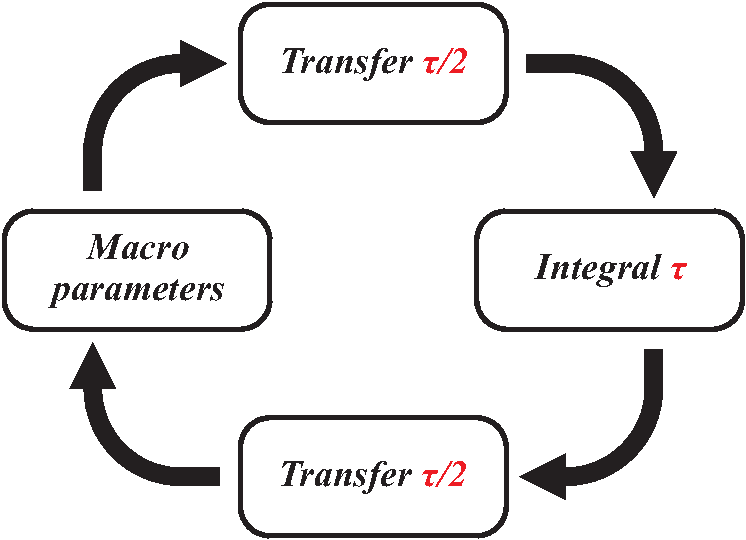
\includegraphics[width=\columnwidth]{pics/split_scheme.pdf}
		\end{column}
	\end{columns}
\end{frame}

\begin{frame}
	\frametitle{Правая часть уравнения Больцмана}
	\begin{itemize}
		\item симметризация по \(\boldsymbol\xi\) и \(\boldsymbol\xi'_1\)
			\[
				J(\boldsymbol\xi_\gamma) = \int\delta(\boldsymbol\xi-\boldsymbol\xi_\gamma)
				(f_1' f' - f_1 f) gb \dd{b} \dd\varepsilon \dd\boldsymbol\xi \dd\boldsymbol\xi_1
			\]
		\item переход от интегрирования к суммированию
			\[ \int\dots\dd{b}\dd\varepsilon\dd\boldsymbol\xi\dd\boldsymbol\xi_1 \to \sum\limits_{\nu=1}^{N_\nu}\dots \]
		\item 8D интегрирующая сетка Коробова \( \{b_\nu,\varepsilon_\nu,\boldsymbol\xi_{\alpha_\nu},\boldsymbol\xi_{\beta_\nu}\} \)
	\end{itemize}
	\begin{block}{}\scriptsize
		Черемисин Ф.Г. \textit{Консервативный метод вычисления интеграла столкновений Больцмана}
			// Доклады РАН. — 1997. — Т. 357, № 1. — С. 53—56.
	\end{block}
\end{frame}

\begin{frame}
	\frametitle{Проекционный метод}
	\begin{columns}
		\begin{column}{4cm}
			\begin{tikzpicture}[scale=.4, >=latex',thick]
				\draw[step=1, gray, very thin] (-5.4,-5.4) grid (5.4,5.4);
				\draw (0,0) circle (5);
				\draw[->] (0,0)--(4,-3) node[below right] {\footnotesize\(\boldsymbol\xi_\alpha\)};
				\draw[->] (0,0)--(-4,3) node[above left] {\footnotesize\(\boldsymbol\xi_\beta\)};
				\draw[->] (0,0)--(4.77,1.5);
				\draw[->] (0,0)--(-4.77,-1.5);
				\pause[2]
				\draw (-5,-2) circle (.1) node[anchor=north] {\footnotesize\(\boldsymbol\xi_{\lambda+s}\)};
				\draw (-4,-1) circle (.1) node[anchor=south] {\footnotesize\(\boldsymbol\xi_\lambda\)};
				\draw (5,2) circle (.1) node[anchor=south] {\footnotesize\(\boldsymbol\xi_{\mu-s}\)};
				\draw (4,1) circle (.1) node[anchor=north] {\footnotesize\(\boldsymbol\xi_\mu\)};
				\pause[1]
			\end{tikzpicture}
		\end{column}
		\begin{column}{6cm}
			\[ 
				\boldsymbol\xi_{\alpha_\nu},\boldsymbol\xi_{\beta_\nu}\in \Omega \rightarrow
				\boldsymbol\xi'_{\alpha_\nu},\boldsymbol\xi'_{\beta_\nu}\notin \Omega 
			\]
			\begin{center}
			\pause[2]
			\alert{Проецирование на \(\Omega\)}\\\smallskip\smallskip
			\begin{tikzpicture}[every node/.style={circle,draw=blue!50,fill=blue!20,thick,inner sep=0pt,minimum size=8mm}, >=latex',thick, node distance=.5]
				\node (alpha) {\footnotesize\(\boldsymbol\xi_\alpha'\)};
				\node (lambda) [below left=of alpha] {\footnotesize\(\boldsymbol\xi_\lambda\)};
				\node (lambdas) [below right=of alpha] {\footnotesize\(\boldsymbol\xi_{\lambda+s}\)};
				\draw [->] (alpha) to (lambda);
				\draw [->] (alpha) to (lambdas);
			\end{tikzpicture}
			\hspace{3mm}
			\begin{tikzpicture}[every node/.style={circle,draw=blue!50,fill=blue!20,thick,inner sep=0pt,minimum size=8mm}, >=latex',thick, node distance=.5]
				\node (beta) {\footnotesize\(\boldsymbol\xi_\beta'\)};
				\node (mu) [below left=of beta] {\footnotesize\(\boldsymbol\xi_\mu\)};
				\node (mus) [below right=of beta] {\footnotesize\(\boldsymbol\xi_{\mu-s}\)};
				\draw [->] (beta) to (mu);
				\draw [->] (beta) to (mus);
			\end{tikzpicture}
			\end{center}
		\end{column}
	\end{columns}
	\pause[3]
	\bigskip\centering \alert{Регуляризация \(f'\) и \(f'_1\)}
	\begin{columns}
		\column{.3\textwidth}
		\begin{block}{\centering с сохранением}
			\begin{itemize}
				\item массы \\
				\item импульса \\
				\item энергии \\
			\end{itemize}
		\end{block}
		\column{.5\textwidth}
		\begin{block}{\centering с нарушением}
			\begin{itemize}
				\item старших моментов \\
				\item молекулярного потенциала \\
			\end{itemize}
		\end{block}
	\end{columns}

\end{frame}

\section{Моделирование}

\begin{frame}
	\frametitle{Разреженный газ между 2 параллельными пластинами}
	\begin{columns}
		\column{.6\textwidth}
		\centering
		\begin{tikzpicture}[dashdot/.style={dash pattern=on .4pt off 3pt on 4pt off 3pt},
							>=latex',thick, scale=1]
			\fill[gray!20] (0,0) -- (3.6,0) -- (3.6,1.5) -- (0,1.5) -- cycle;
			\draw[dashdot] (-.2,0) -- (3.8,0);
			\draw[very thick] (0,1.5) -- (3.6,1.5);
			\draw[<->] (.7,0) -- (.7,.75) node[left] {\(\dfrac{L}{2}\)} -- (.7,1.5);
			\draw[<->] (3.2,0) node[above] {\(y\)} -- (2.4,0) -- (2.4,.8) node[right] {\(x\)};
		\end{tikzpicture}\\
		\bigskip
		\begin{itemize}
			\item одномерная задача \\
			\item линейная \(\left|\frac{\partial \hat{h}_i}{\partial x_i}\right| \ll 1 \) \\
			\item диффузное отражение \(\alpha=1\) \\
			\item одноатомный идеальный газ \\
			\item модель твердых сфер \\
		\end{itemize}
		\column{.5\textwidth}
		\setbeamertemplate{items}[circle]
		\setbeamerfont{item projected}{size=\large}
		\setbeamerfont{itemize/enumerate body}{size=\large}
		\begin{enumerate}
			\item течение Куэтта \\
			\item перенос тепла \\
			\item течение Пуазёйля \\
			\item тепловая транспирация \\
		\end{enumerate}
	\end{columns}
\end{frame}

\begin{frame}
	\frametitle{Течение Куэтта и перенос тепла}
	\begin{columns}
		\column{.55\textwidth}
		\begin{center}
			Сдвиговое напряжение\\
			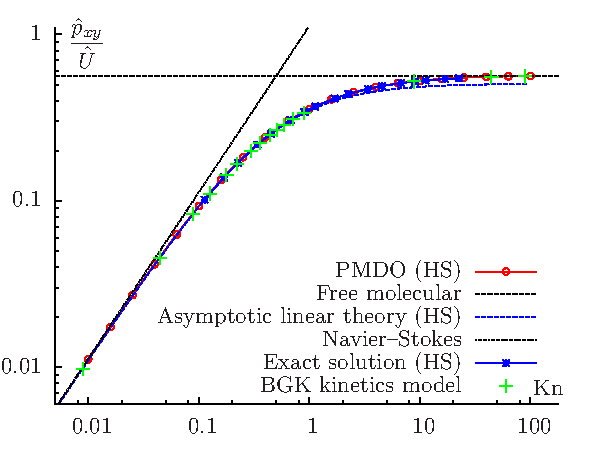
\includegraphics[width=\textwidth]{pics/couette_stress}
		\end{center}
		\column{.55\textwidth}
		\begin{center}
			Поток тепла\\
			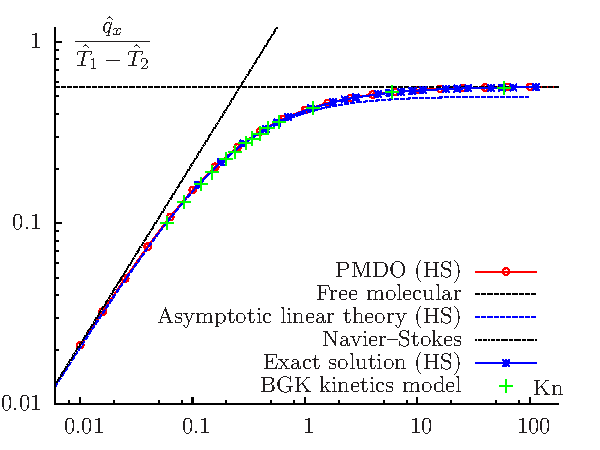
\includegraphics[width=\textwidth]{pics/heat_qflow}
		\end{center}
	\end{columns}
\end{frame}

\begin{frame}
	\frametitle{Исследование погрешности}
	\begin{columns}
		\column{.8\textwidth}
		\begin{center}
			Значение относительной ошибки\\
			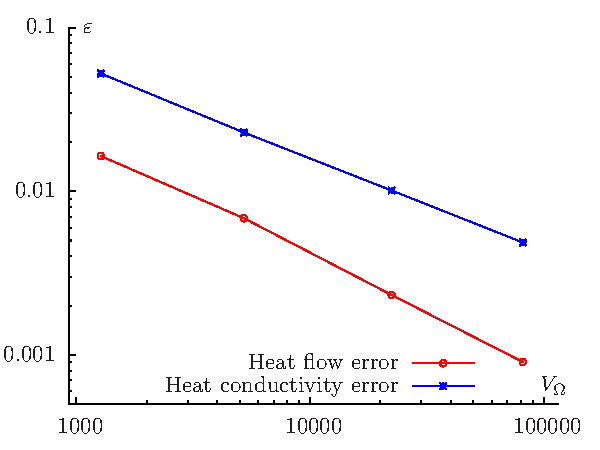
\includegraphics[width=\textwidth]{pics/error}
		\end{center}
		\column{.2\textwidth}
		\begin{center}
			Сходимость \alert{2/3} порядка по \alert{объёму} скоростной сетки
		\end{center}
	\end{columns}
\end{frame}

\begin{frame}
	\frametitle{Продольные потоки}
	\begin{columns}
		\column{.55\textwidth}
		\begin{center}
			Поток через половину сечения\\
			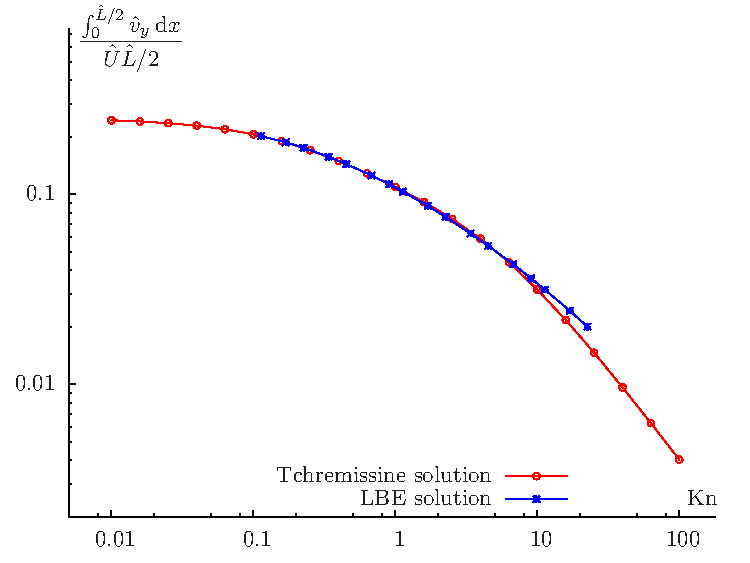
\includegraphics[width=\textwidth]{pics/couette_flow}
		\end{center}
		\column{.55\textwidth}
		\begin{center}
			Продольный поток тепла\\
			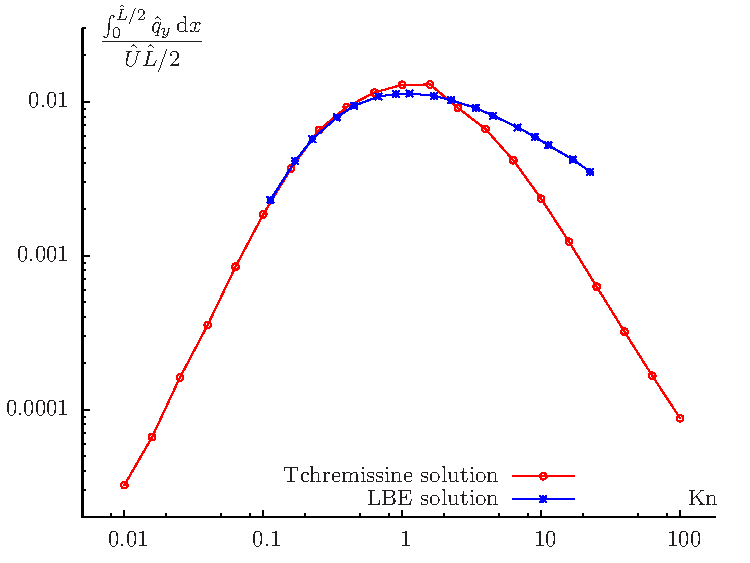
\includegraphics[width=\textwidth]{pics/couette_qflow}
		\end{center}
	\end{columns}
\end{frame}

\begin{frame}
	\frametitle{История решения задачи Пуазёйля}
	\begin{itemize}
		\item \textit{James Clark Maxwell, 1879} \\ формулировка условий скольжения газа вдоль стенок \\
		\item \textit{Martin Knudsen, 1909} \\ экспериментальное определение минимума потока газа \\
		\item \textit{Carlo Cercignani, 1963} \\ первое численное решение на основе кинетического уравнения БКВ \\
		\item \textit{Taku Ohwada, Yoshio Sone, Kazuo Aoki, 1989} \\ точное решение задачи для модели твёрдых сфер \\
		\item \textit{Timothee Ewart et al., 2007} \\ прецизионный эксперимент для широкого диапазона чисел Кнудсена \\
	\end{itemize}
\end{frame}

\begin{frame}
	\frametitle{Верификация 2D решения}
	\begin{center}
		Поток через сечение\\
		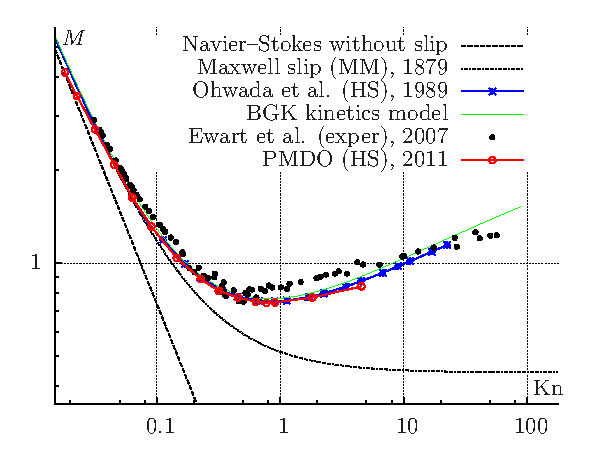
\includegraphics[width=.8\textwidth]{pics/poiseuille}
	\end{center}
\end{frame}

\section*{}
\begin{frame}
	\frametitle{Заключение}
	\begin{itemize}
		\item \alert{второй порядок} сходимости по координатам и по радиусу скоростной сетки \\
		\item \alert{верификация} численного метода на основе линейной теории (\(\mathrm{Re}\ll1\)):
		\begin{itemize}
			\item 1D решение задачи Куэтта
			\item 2D решение задачи Пуазёйля
		\end{itemize}
	\end{itemize}
\end{frame}


\end{document}
